%%%%%%%%%%%%%%%%%%%%%%%%%%%%%%%%%%%%%%%%%%%%%%%%%%
%% Bachelor's & Master's Thesis Template        %%
%% Copyleft by Dawid Weiss & Marta Szachniuk    %%
%% Faculty of Computing and Telecommunication   %%
%% Poznan University of Technology, 2020        %%
%%%%%%%%%%%%%%%%%%%%%%%%%%%%%%%%%%%%%%%%%%%%%%%%%%


% Szkielet dla pracy licencjackiej pisanej w języku polskim.

\documentclass[english,bachelor,a4paper,oneside]{ppfcmthesis}


\usepackage[utf8]{inputenc}
\usepackage[OT4]{fontenc}

% Fix footnotes to the bottom of the page
\usepackage[bottom]{footmisc}

% Better table formatting
\usepackage{makecell}               % Makecell for breaking a long text
\renewcommand{\cellalign}{tl}       % Makecell left alignment
\renewcommand{\arraystretch}{1.75}  % More vertical padding

%--------------------------------------
% Strona tytułowa
%--------------------------------------

% Autorzy pracy, jeśli jest ich więcej niż jeden
% wstaw między nimi separator \and
\author
{%
   Patryk Kościk \album{144635}
}
\authortitle{}                                % Do not change.

\title
{%
   Performance analysis of different emulation methods 
   in control systems and IoT devices on the example of
   the Renode Framework
}

% Your supervisor comes here.
\ppsupervisor{dr inż.~Adam Turkot} 

% Year of final submission (not graduation!)
\ppyear{2023}                                 


\begin{document}

% Front matter starts here
\frontmatter\pagestyle{empty}%
\maketitle\cleardoublepage%

%--------------------------------------
% Miejsce na kartę pracy dyplomowej
%--------------------------------------

\thispagestyle{empty}\vspace*{\fill}%
\begin{center}Tutaj będzie karta pracy dyplomowej;\\oryginał wstawiamy do wersji dla archiwum PP, w pozostałych kopiach wstawiamy ksero.\end{center}%
\vfill\cleardoublepage%

%--------------------------------------
% Spis treści
%--------------------------------------

\pagenumbering{Roman}\pagestyle{ppfcmthesis}%
\tableofcontents* 
\cleardoublepage % Zaczynamy od nieparzystej strony

%--------------------------------------
% Rozdziały
%--------------------------------------

%Najwygodniej jeśli każdy rozdział znajduje się w oddzielnym pliku
\mainmatter%

\chapter{Introduction}

In a embedded devices development context, platform simulation is referring to a method of simulating 
the behavior of an entire platform, or only a few selected components, in order to test and evaluate
the functionality and performance of the system before it is deployed. This can be done using specialized
software tools and techniques that simulate the hardware, software, and other components of the platform,
allowing developers to run and test their code in a virtual (simulated) environment before it is implemented
onto the physical hardware.

Platform simulation became an indispensable tool in the modern-day embedded system development. Such technology
provides each engineer with an dedicated, deterministic and reproducible system for development, testing and debugging.
This approach allows the developers to use advanced debugging software to perform a wide range of tests to ensure that
the embedded system is functioning correctly and meeting the desired performance and reliability requirements. 
This allows developers to detect, identify and fix bugs early in the development process, saving time and resources.

The advantages of the platform simulation also reach beyond the software development phase, and well into the further
phases of the product lifespan. One such advantage is the ability to easily integrate these systems into existing
continuous integration (CI) systems that check for regressions with each software/hardware iteration.
This is because the entire platform is contained within a simulation layer, making integration much simpler than it
would be with hardware platforms, which would require a hardware/software integration layer. An another example of
the benefit brought by emulation is an ability to create software, without having an hardware platform ready.
This is an especially important in the post COVID-19 pandemic times, where the supply chains have been massively
disrupted, with lead time on some parts, especially for the most advanced elements, rising as much as four times,
from about four weeks, in the begging of the year 2020, to over twenty weeks at the end of 2021
\cite{Covid19-AUTOMOTIVE} \cite{Covid19-LEAD-TIME} \cite{Covid19-LEAD-TIME-BLOOMBERG}. Hardware emulation allows for
the parallelization of the software and hardware development, enabling developers to work on both aspects
simultaneously and reducing the overall time and effort required to bring a product to market.

\section{Motivation and goals of the thesis}

A large part of the recognized platform and/or core architecture emulators use opcode translation to run guest code
on the host platform. The most prevalent and widely used open source tools in this category include Renode \cite{Renode}
and QEMU \cite{Qemu}.%
\footnote{The Renode's CPU translation library is partly based on QEMU}
Due to major optimizations (translation blocks, caching, block chaining, ...), this method of the simulation yields
great results performance-wise, but on the other hand such heavy efficiency improvements come with a price of greatly 
complicating the codebase, making it difficult to maintain and integrate new functionality. Another downside of the
translation based approach is the need to \textbf{execute} the guest code, this requires complicated just in
time (\textit{JIT}) recompilers. A possible alternative to translation based CPU simulators are the interpretation
based CPU simulators. This approach tend to be much simpler as these simulators do not require code recompilation,
and usually do not implement very complicated optimizations, instead focusing on simple, maintainable and easily
expandable implementation of the simulated core instructions. While the lack of optimizations results in simpler
code, the simulation performance might suffer.

The main goal of the thesis is to integrate an already existing interpretation-based CPU simulator within the Renode
embedded system simulation framework. Then to compare the performance and accuracy of the simulation using benchmarks
and real world applications such as automatic control systems, general purpose real-time operating systems 
\textit{(RTOS)}, and even higher complexity binaries, for example AI solutions for the embedded devices.
By doing so, we hope to gain a better understanding of the performance capabilities and limitations of this approach,
and to identify potential areas for improvement and future work in this topic.

% Not indenting here as this is connected to the previous paragraph
\noindent Intermediate goals of the thesis include:
\begin{itemize}
	\item{Description of the existing translation and interpretation based approach CPU simulators}
	\item{Integrating an chosen interpretation CPU simulator into the Renode framework}
	\item{Implementation of the test software on the simulated platform with data gathering}
	\item{Comparative analysis of interpreter-based and translation-based solutions with regard to the performance}
\end{itemize}

\section{Thesis organization}

The work is divided into the following chapters:
\begin{itemize}
	\item{Chapter 2 will provide an in-depth description of the Renode's translation CPU simulation library}.
	\item{Chapter 3 provides an overview of Dromajo, the chosen simulation library}.
	\item{Chapter 4 focuses on integrating Dromajo into the Renode framework}.
	\item{Chapter 5 describes the benchmarks and the test binaries and presents their results}.
	\item{Chapter 6 concludes the thesis and suggests future work}.
\end{itemize}

\chapter{Simulation basics}

In computing, a simulator is a software program that aims to simulate or emulate the behavior of a system or a component.
Central processing unit simulation refers to the subset of simulators that aim to emulate the functionality and
characteristics of the device processor.

% image here showing the guest and host with the simulation layer in between them
\begin{figure}[h]
	\centering
	\vspace{10px}
	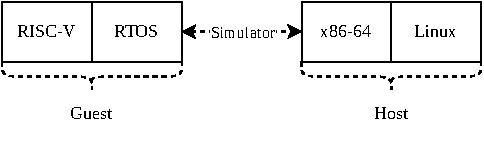
\includegraphics[height=90px]{figures/GuestHostSimulator.pdf}
	\caption{Guest and host with the simulation layer in between}
\end{figure}

% it would be great if you referenced this image in text. Add a \label within the figure, and \ref in text

The machine running the simulator is called the host system, while the simulated system is called the guest or the target
system. The target system instruction set architecture is most often, but not necessarily, different from the host
architecture. The simulator complexity can vary significantly in the domain of complexity and detail.
The extent of the simulation and its verbosity is largely determined by the specific requirements of the application.

According to the Austin et. al \cite{Simplescalar}, three fundamental factors describing the simulator requirements are:

\begin{itemize}
	\item{\textbf{Performance} is the measure of how fast the simulator can finish the specific workload. This metric
	can be described in many ways. One of them being the most intuitive measure of a \textit{relative slowdown/speedup}
	describing the ratio of the time it takes to execute a workload on a simulated hardware, to the time spent
	executing the same workload on the hardware.}
	%
	\item{\textbf{Detail} determines the accuracy of the simulator's state replication in the relation to the hardware,
	which can be described in the terms of how many layers of abstractions are implemented.}
	%
	\item{\textbf{Flexibility} indicates the adaptability of a design. This takes into account factors such as
	portability, modularity, ease of implementing new features, exposed APIs, and many other factors.}
\end{itemize}

It is very difficult to maximize all three of these aspects, and this is the reason why there are so many simulation
solutions available. Most research models tend to optimize performance and flexibility at the expense of detail
\cite{Simplescalar}.

\pagebreak
\section{CPU simulation techniques}

The central processing unit can be simulated in various ways. Each of these simulation methods aims to achieve the same
objective, but employs a distinct approach to the problem. N. Srivastava lists \cite{Nitish-Techniques} these methods:

\begin{itemize}
	\item{\textbf{Functional simulation}, also called an \textbf{Instruction set simulation}, focuses only on the
	fundamental characteristics of the design and correctness of the simulated instruction set architecture,
	% my proposition of slightly changing it.
	i.e. answers the question: "Does this software behave as expected on a given architecture?". Such simulators do not implement any
	timing functionality, and cannot be used to gauge the performance of the simulated architecture. An example of such
	a simulator is Spike, a RISC-V ISA Simulator \cite{Spike}.}
	%
	\item{\textbf{Trace driven simulation}, this type of simulator uses a prerecorded session (\textit{trace}), that is
	later used to simulate the CPU behavior. The trace can be generated either by an existing hardware device or
	using software-based techniques, such as hardware monitoring, binary instrumentation, or trace synthesis
	\cite{Simplescalar}. This method has numerous benefits, such as full determinism, as the whole simulation is
	encapsulated in the trace file. However, since such simulators are limited to simulating traces, they
	cannot easily run arbitrary code. Additional disadvantages of this approach are the requirement for a large
	amount of data storage space, and the poor performance when simulating parallel or timing-dependent systems
	\cite{TraceDrivenAccuracy}. An example of such simulator is gem5 \cite{gem5}, specifically, the \textit{TraceCPU}
	and \textit{Elastic Traces} \cite{gem5trace}.}
	%
	\item{\textbf{Execution driven simulation}, these simulators combine timing and functionality together
	\cite{Nitish-Techniques}, by \textit{executing} the guest instructions, as if they were executed on the hardware.
	This is achieved by translating or interpreting the guest binary code, to the host code (or if the guest
	architecture matches the host's architecture, directly executing the code). Since no traces are needed, the
	% While referencing Hennessy is always a good idea, what do you mean by one machine? As opposed to what?
	simulation can be performed without a trace generator, using only one machine \cite{TraceDrivenAccuracy}.
	The accuracy of the simulation is exclusively determined by the accuracy of the simulator, and the levels of
	abstraction chosen by the simulator developers. Examples of such simulators are the beforementioned QEMU and
	% I assume you also include Renode here? We can't really say "qemu is here, so Renode is automatically covered", Renode is far from being qemu++.
	Dromajo \cite{Dromajo}.}
\end{itemize}

This work will focus solely on the \textbf{execution driven simulators}, but it is important to understand the
different approaches and their purpose. The table \ref{tab:simulators} summarizes this classification:

% frankly i'm not a great fan of this distinction, but naming is not a settled thing, so I won't object
\begin{table}[h]
	\centering
	\begin{tabular}{l|l}
	Type 				& Purpouse 																			 \\ \hline
	Functional 			& \makecell{Validate and verify the correctness of the instruction set architecture} \\ \hline
	Trace 				& \makecell{Simulate the architecture and performance of the processor} 			 \\ \hline
	Execution driven 	& \makecell{Simulate the actions of a processor, rather than the underlying \\
									mechanisms by which it performs those actions}
	\end{tabular}
	\caption{Simulation types}
	% ref needs to go after a caption. Always have them anyway
	\label{tab:simulators}
\end{table}

\pagebreak
\section{Execution driven CPU simulators}

Execution driven simulators can be further divided into two distinct types:

\begin{itemize}
	\item{\textbf{Translation simulators} use dynamic, just-in-time (\textit{JIT}) recompilation of the binary.
	When simulating a CPU architecture that differs from that of the host system,%
	\footnote{If the host and guest architectures match, the translation process can, but does not have to, be skipped,
	by implementing virtualization mechanisms, such as QEMU's KVM \cite{QemuKVM}, or other hypervisor based approaches.}
	% "involves" appears a lot in this paragraph. Not an error, but you might want to reword it a little
	the process of executing guest code involves two phases. The first phase involves interpreting the guest code into
	an intermediate (architecture-independent) representation. The second phase involves recompiling the intermediate
	code into host architecture code, which is subsequently executed on the host's CPU. This process is called
	\textit{Dynamic Binary Translation}, often referred to simply as \textit{translation}.%
	\footnote{While the intermediate code representation is \textit{not} necessary, it allows for a greater degree of
	flexibility and portability.}

	The translated code can be organized into blocks called \textit{Translation Blocks}, which can be cached and
	% this citation is not very specific... I would rather refer to your chapters (with \ref), where you describe both concepts
	chained \cite{Qemu}.

	Such optimizations greatly improve the performance (\textit{redcuce the relative slowdown}), at the
	cost of a complicated simulator codebase. Moreover, this technique implies limited portability, as there is a need
	to implement a new recompiler for each host CPU architecture.

	This method of execution driven simulation will be described thoroughly in Chapter 3, on the example of Renode's
	\textit{Translation library} \cite{Tlib}.}
	%
	\item{\textbf{Interpretation simulators} work by \textit{interpreting} the guest binary. Firstly the simulator
	reads (\textit{fetches}) the opcode, then parses (\textit{executes}) said opcode according to the ISA standards.
	The execution is implemented as a modification of an internal CPU state, which is stored in memory as a data type,
	describing the CPU features and state, such as registers, exception flags, etc.

	% well, it DOES execute code, but not the one it generates
	Since this type of simulator \textbf{does not} does not generate any code for execution on the host's CPU, the recompilation step is not
	necessary. This greatly simplifies the simulator codebase and increases portability. On the other hand, the lack of
	features, such as translation blocks, makes various optimization techniques not possible.

	One example of such a simulator is Dromajo \cite{Dromajo}. The details of its implementation will be described in
	Chapter 4.}
\end{itemize}


\section{Whole-system simulation}

To fully understand the topic of simulation, the reader must also grasp the concept of whole-system simulators. Whole
system simulators implement a beforementioned CPU simulator, alongside peripheral support. Peripherals might be
modeled as a simulation element, or might be passed through to a physical, hardware device. For example, the peripheral
equipment for an embedded system might consist of:
\begin{itemize}
	\item{Serial interfaces,}
	\item{General-purpose input/output,}
	\item{Communication devices, such as I$^2$C, SPI and network controllers.}
\end{itemize}

\pagebreak
\section{Other notable simulators types}

The definition of simulation is broad and extends beyond system emulation. Solutions such as WINE, VMWare Workstation
and QEMU user-mode emulation focus on distinct goals and approaches:

\begin{itemize}
	\item{\textbf{WINE}, recursive backronym for \textit{Wine Is Not an Emulator} \cite{Wine}, is essentially an MS
	Windows API wrapper. This simulator does not attempt to emulate the underlying architecture of the hardware.
	Instead, it focuses on solely simulating software-defined system calls (\textit{syscalls}).}
	%
	\item{\textbf{VMWare Workstation} \cite{VMWareWorkstation} and \textbf{VirtualBox} \cite{VirtualBox}, both of these
	focus on system emulation, but their emulation scope is focused only on simulating an x86 and AMD64/Intel64 machines.
	They operate on the principle of virtualization, to create so-called \textit{virtual machines}. Virtualization
	software directly executes unprivileged code on the host processor. If the host's processor does not support
	x86 virtualization extensions, such as Intel's \textit{VT-x} or AMD's \textit{AMD-V}, the privileged code is firstly
	translated, and then ran on the host. If the host's CPU supports the beforementioned extensions, the guest code does
	not need to be translated.

	Both of mentioned software are referred to as \textit{Level 2 Hypervisors}, as they run on top of the host
	operating system. There are also commercial and open source \textit{Level 1 Hypervisors}, behaving
	as an operating system that is used to provide better guests performance, by the means of providing better and more
	performant access to the underlying hardware \cite{Graniszewski_Waldemar_Performance_2016}.}
	%
	\item{\textbf{QEMU user-mode}, this solution enables the execution of binaries compiled for a different CPU
	architecture on the host system. This approach not only translates the code from the guest to the host but
	additionally translates system calls, handles POSIX signals, and enables proper threading support
	\cite{QemuUser}.

	This solution is useful when creating and debugging Linux and BSD-based applications intended for embedded devices}
\end{itemize}

Unfortunately, these methods of simulation are unsuitable for the creation and testing of embedded devices due to their
restrictive nature and limited capabilities. In particular, their inability to simulate other architectures, limited
% avoid big quantifiers, or you'll have to defend them
debugging capabilities, and lack of customizability for system peripherals make them difficult to be utilized in this
context.

\section{Conclusions}

In this chapter, we briefly examined the existing CPU simulation techniques and their purposes. We divided execution
driven simulators into two distinct types, described the process of the whole system simulation, 
% what do you mean by "and example peripheral in the context of embedded devices"?
and example peripheral
in the context of embedded devices, finally, we finished by mentioning other noteworthy simulators.

Overall, for most cases, the Execution-driven CPU simulator combined with a whole-system emulation framework will be the
most suitable option for most IoT and embedded device development teams, as it provides the needed flexibility, is able
to run arbitrary workloads, and can provide an in-depth look at the guest system.

The hypervisor and syscalls emulators are not functionality rich enough to demonstrate their value in the IoT and
embedded devices development cycle where direct interaction with the hardware layer is an important part of the programmer's work.

%--------------------------------------
% Literatura
%--------------------------------------

\bibliographystyle{unsrt}{\raggedright\sloppy\small\bibliography{bibliografia}}

%--------------------------------------
% Dodatki
%--------------------------------------

\cleardoublepage\appendix%
\newpage
% Removing all includes from this section breaks some conditional
\if

%--------------------------------------
% Informacja o prawach autorskich
%--------------------------------------

\ppcolophon

\end{document}
